\begin{figure}[t]
  \centering
  \begin{tikzpicture}
    \node[inner sep=0pt] (map) at (0, 0)
         {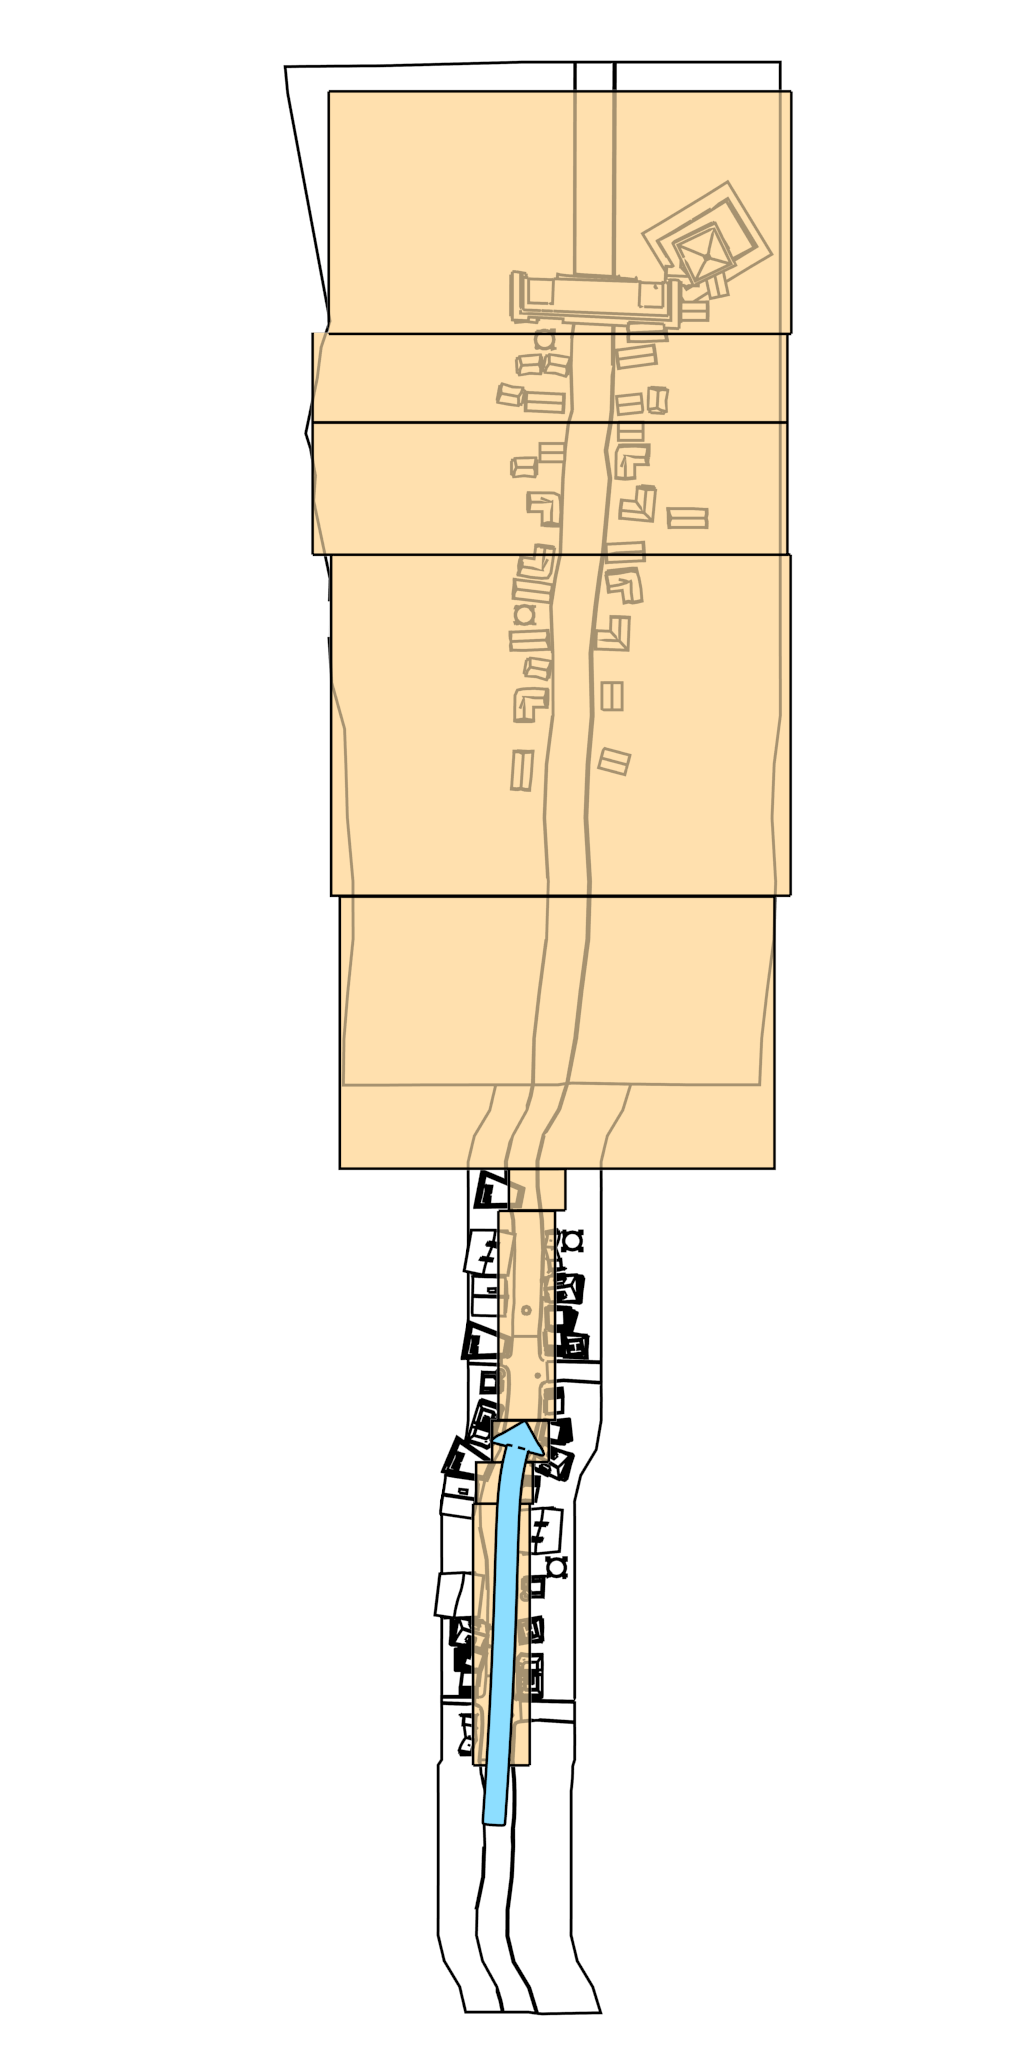
\includegraphics[width=\textwidth]{./img/raw/test-suite-pipers-alley-map.png}};
    \node[inner sep=0pt] (map) at (0.0\textwidth, 0.05\textwidth) 
         {
\includegraphics[width=\textwidth]{./img/raw/test-suite-pipers-alley-map-size.png}};
    \node (l3) at (0.415\textwidth, -0.15\textwidth) {$90$ eenheden};
  \end{tikzpicture}
  \caption{Een overzicht van de Piper's Alley scene.}
  \label{fig:test-suite-pipers-alley-map}
\end{figure}

